\documentclass[lettersize,journal]{IEEEtran}
\usepackage{amsmath,amsfonts}
\usepackage{algorithmic}
\usepackage{algorithm}
\usepackage{array}
\usepackage[caption=false,font=normalsize,labelfont=sf,textfont=sf]{subfig}
\usepackage{textcomp}
\usepackage{stfloats}
\usepackage{url}
\usepackage{verbatim}
\usepackage{graphicx}
\usepackage{cite}
\graphicspath{{../figures/}}
\hyphenation{op-tical net-works semi-conduc-tor IEEE-Xplore}

\begin{document}

\title{DualCMP: Cooperative Motion Prediction with Fused and Source-Specific BEV Representations}

% Author names and affiliations are not specified in manuscript.md.
\author{}

\maketitle

\begin{abstract}
Predicting the future motion of surrounding agents is essential for safe autonomous driving. Vehicle-to-everything communication improves scene understanding by sharing observations from spatially separated connected and automated vehicles (CAVs). Existing cooperative predictors mainly fuse BEV features for perception or associate tracked trajectories before forecasting. These pipelines improve scene understanding and historical motion representation, respectively. Motion prediction, however, often relies on agent-specific spatial context, and the informative viewpoint may vary across agents because of sensing range and occlusion. We propose \textbf{DualCMP}, a cooperative motion prediction framework that uses fused and source-specific BEV features. DualCMP uses the same LiDAR encoding in two ways: fused BEV features update persistent agent queries, while each query aggregates local features from the aligned CAV feature maps. A motion-anchored decoder integrates the cooperative context with motion history and agent interactions to generate multimodal trajectories. Under strict-online evaluation on V2V4Real, the current seed-20 model obtains a 5-s minADE$_6$ of 1.9350 m and minFDE$_6$ of 3.2465 m; attention analysis further shows that its CAV weights vary with observation support and relative geometry. A protocol-matched fused-BEV comparison is still required to attribute a forecasting gain to the source-specific representation.
\end{abstract}

\begin{IEEEkeywords}
Cooperative perception, motion prediction, vehicle-to-everything communication, persistent queries, bird's-eye-view representation.
\end{IEEEkeywords}

\section{Introduction}
\IEEEPARstart{M}{otion} prediction is a core component of autonomous driving because safe planning depends on anticipating the future motion of surrounding agents \cite{zhou2022hivt,zhou2023qcnet}. A predictor uses observed agent states, neighboring agents, and local scene context to generate multiple plausible futures, while occlusion, sparse LiDAR returns, and limited sensing range can make the inputs incomplete \cite{zhou2022hivt,zhou2023qcnet}. Vehicle-to-everything communication provides the receiver with observations from spatially separated connected and automated vehicles (CAVs) \cite{xu2023v2v4real,wang2020v2vnet}. After spatial alignment, CAV observations can extend the receiver's line of sight and supply complementary context for scene understanding and forecasting \cite{wang2020v2vnet,zhou2025v2xpnp}. When forecasting begins, the choice of representation determines which cooperative evidence remains available for a particular target agent.

Existing cooperative motion-prediction methods use CAV observations at different stages and provide different representations to downstream modules. Intermediate-fusion methods encode and align CAV BEV features before detection and tracking, so downstream modules receive a fused BEV for receiver-side scene understanding \cite{wang2020v2vnet,wang2025cmp,zhou2025v2xpnp}. By combining observations from multiple viewpoints in a common frame, the fused BEV representation supports current-state estimation. A second line of work starts from detections, tracks, or historical trajectories produced by separate perception streams and performs cross-view association or trajectory fusion before forecasting, whereas prediction-level methods combine forecast hypotheses produced by separate predictors \cite{yu2023v2xseq,ruan2024v2xgraph,wu2025copad,zhang2025comtp,wang2025cmp,madjid2026latefusion}. Later fusion stages preserve view-specific motion histories or forecast hypotheses, but dense spatial observations have already been converted into boxes, tracks, or trajectory features before the final cooperative representation is formed. Fig.~\ref{fig:introduction} summarizes the main distinction: intermediate fusion forms the fused BEV before agent-state estimation, whereas trajectory fusion begins with view-specific histories after perception and tracking.

\begin{figure}[!t]
\centering
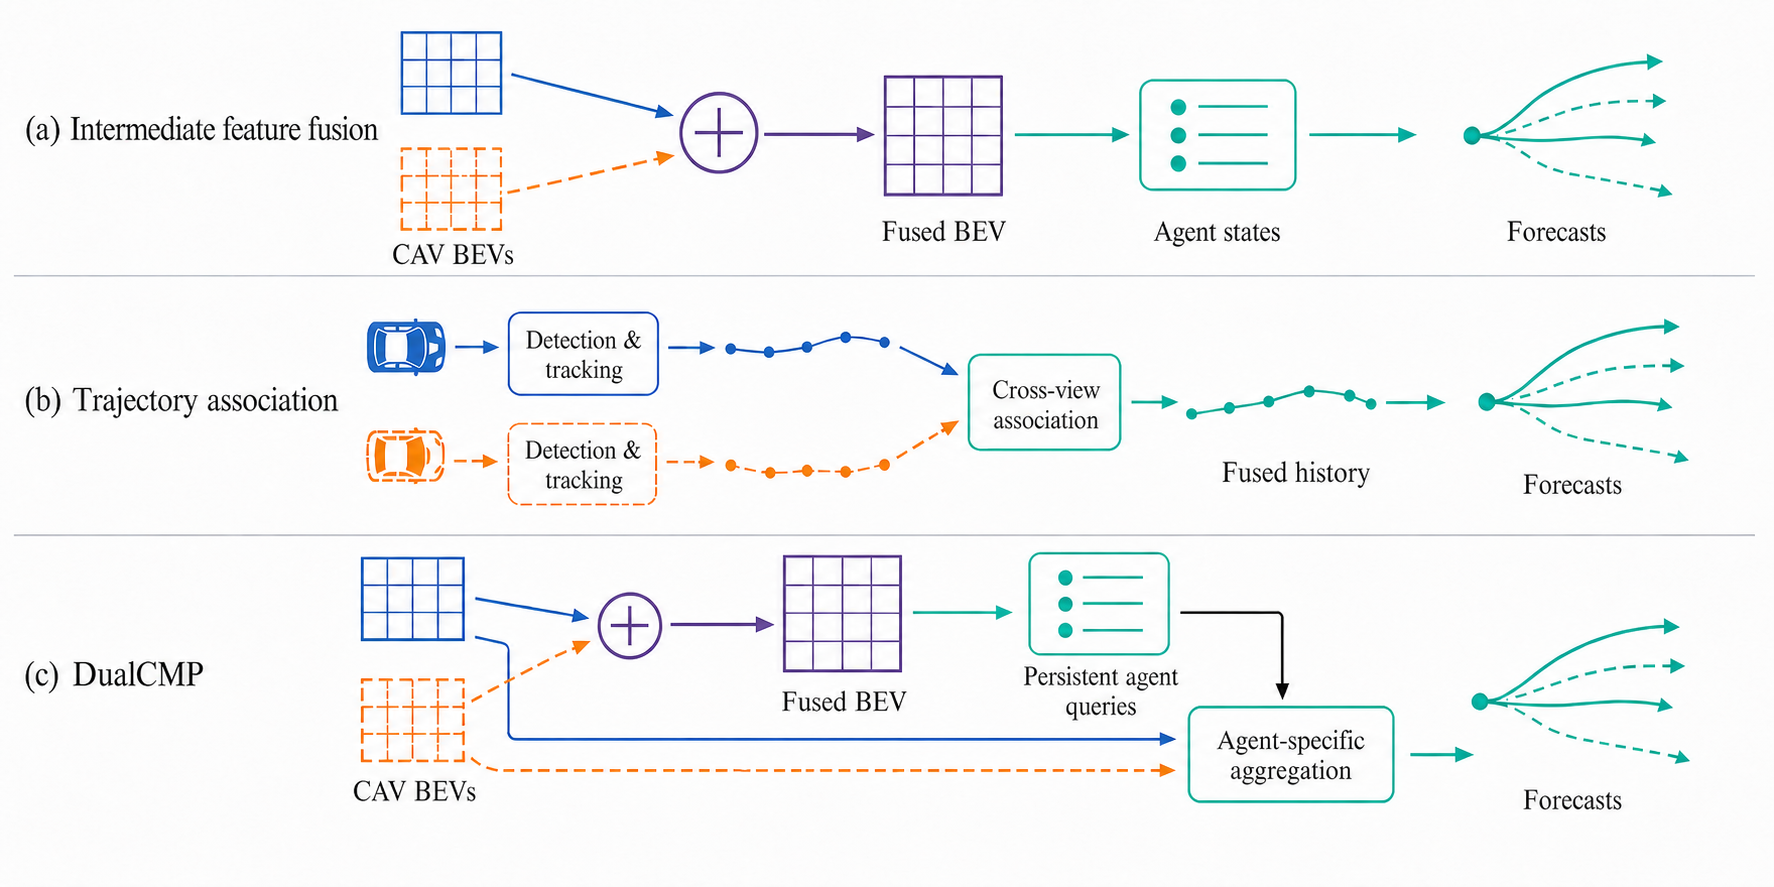
\includegraphics[width=\columnwidth]{dualcmp_introduction_fig1_v3}
\caption{Cooperative information fusion for motion prediction. (a) Intermediate fusion aggregates aligned CAV BEV features before agent-state estimation and forecasting. (b) Trajectory fusion associates and fuses histories generated by separate detection and tracking pipelines before forecasting. (c) DualCMP uses fused BEV features to update persistent agent queries and aggregates aligned CAV feature maps for agent-centric motion prediction.}
\label{fig:introduction}
\end{figure}

For motion forecasting, the predictor organizes motion history, neighboring agents, and local context around a particular target agent \cite{zhou2022hivt,zhou2023qcnet}. The relevance of different viewpoints can vary across target agents because each agent has a different spatial relation to the observing CAVs. A viewpoint that supplies useful evidence for one agent may be less informative for another agent in the same scene \cite{wang2025cmp,ruan2024v2xgraph}. Intermediate fusion preserves spatial context in the fused BEV, but the source dimension is no longer explicit when a common agent state is formed. Trajectory- and prediction-level fusion preserve view-specific histories or locally generated forecast hypotheses, but their cooperative representations do not expose the dense, receiver-aligned CAV maps after the target reference is established. The resulting interfaces therefore do not allow a downstream predictor to retrieve source-specific spatial features for a particular target, although the common scene representation remains useful for current-state estimation.

To address the limitation, DualCMP retains both representations from a shared LiDAR encoder. FuseBEVT aggregates the aligned CAV BEV features into a fused BEV and uses it to update one persistent query for each traffic agent. After the query is formed, the motion predictor uses the query and its current box as a target reference to retrieve local features from the aligned CAV maps and combines them with relative CAV--agent geometry. The resulting design keeps current-state estimation receiver-centric while providing agent-specific multi-view spatial context for forecasting without maintaining separate tracks for individual CAVs. A motion-anchored decoder combines the cooperative context with ordered motion history and inter-agent interactions to generate multimodal trajectories. Because persistent queries can contain different amounts of observed history and state estimates can be noisy, the decoder derives trajectory anchors from the observed history and predicts residual trajectories around them. We evaluate the complete model under a strict-online protocol and use a fixed-tracking comparison between fused and per-CAV forecasting inputs to test the contribution of source-specific spatial features.

The main contributions are summarized as follows:
\begin{enumerate}
\item We present a receiver-side cooperative motion prediction framework that processes online multi-CAV LiDAR observations, updates persistent agent queries from fused BEV measurements, and forecasts from the online states rather than precomputed tracking trajectories.
\item We develop agent-specific CAV feature aggregation that retrieves local aligned BEV features conditioned on the target query and relative CAV--agent geometry, while sharing one LiDAR encoder and keeping a single receiver-side state for each agent.
\item We introduce a motion-anchored forecasting pipeline and a fixed-tracking evaluation that jointly reports tracking, forecast coverage, and trajectory accuracy for matched agent sets under fused and per-CAV forecasting inputs.
\end{enumerate}

The remainder of the paper is organized as follows. Section II reviews related work. Section III defines the cooperative motion prediction problem, Section IV presents DualCMP, and Section V reports the experimental results.

\section{Related Work}
\subsection{Cooperative Perception and Prediction}

Cooperative perception methods exchange raw observations, object outputs, or intermediate features to improve receiver-side scene understanding. Intermediate fusion balances spatial context and communication cost and is the perception backbone used by CMP \cite{wang2025cmp}. CMP extends cooperative perception to motion prediction through a modular detection--tracking--prediction pipeline and a second exchange of predicted trajectories. V2XPnP studies one-step spatio-temporal fusion for end-to-end multi-agent perception and prediction \cite{zhou2025v2xpnp}, while UniMM-V2X uses perception-level and prediction-level cooperation with task-specialized representations \cite{souig2026unimm}.

Trajectory-level methods instead start from historical trajectories produced by upstream perception and tracking. PP-VIC fuses vehicle and infrastructure trajectories with CBMOT before applying a trajectory predictor \cite{yu2023v2xseq}. V2X-Graph learns cross-view associations and fuses motion and interaction features \cite{ruan2024v2xgraph}; CoPAD combines Hungarian matching with Kalman filtering for multi-source trajectory fusion \cite{wu2025copad}; and Co-MTP performs trajectory fusion over history and future domains \cite{zhang2025comtp}. ViTraj further learns vehicle-side and infrastructure-side trajectory representations \cite{you2025vitraj}. Prediction aggregation provides a later form of cooperation in CMP and in recent late-fusion work \cite{wang2025cmp,madjid2026latefusion}. DualCMP retains intermediate fusion for persistent state estimation and reuses the aligned CAV feature maps for agent-centric motion prediction.

\subsection{Agent-Centric Motion Forecasting}

Motion predictors commonly combine temporal agent states, local scene context, and social interaction. HiVT separates local context extraction from global agent interaction and uses relative geometric representations \cite{zhou2022hivt}. QCNet uses query-centric encoding and a proposal--refinement decoder in which proposed trajectories provide adaptive anchors for context retrieval \cite{zhou2023qcnet}. DualCMP adopts neither model directly: V2V4Real provides no HD map in the current setup, and DualCMP inputs are online persistent-query states rather than ground-truth trajectory histories. We instead use their architectural principles to organize observed motion history, relative CAV geometry, agent interaction, and multimodal decoding.

\subsection{Joint Tracking and Forecasting}

Persistent object queries have been used to connect detection, tracking, and forecasting in single-vehicle systems. Predicted motion can also support occlusion handling or subsequent perception in methods such as PF-Track and ForeSight \cite{pang2023pftrack,papais2025foresight}. DualCMP instead uses persistent queries to maintain agent identity and treats forecasting as a read-only consumer of the online tracking state.

\section{Problem Formulation}

Consider a scene with \(N_t\) available CAVs at time step \(t\), and let \(r\in\{1,\ldots,N_t\}\) denote the receiver. We denote the LiDAR point cloud and pose of CAV \(j\) by \(\mathbf{L}_t^j\) and \(\boldsymbol{\xi}_t^j\), respectively. The relative transformation from CAV \(j\) to receiver \(r\) and the runtime input are
\[
\mathbf{T}_{j\rightarrow r}^t
=\left(\boldsymbol{\xi}_t^r\right)^{-1}\boldsymbol{\xi}_t^j,
\qquad
\mathcal{X}_r^t=
\left(
\left\{\mathbf{L}_t^j,\mathbf{T}_{j\rightarrow r}^t\right\}_{j=1}^{N_t},
\boldsymbol{\xi}_t^r,\tau_t^r
\right),
\tag{1}
\]
where \(\tau_t^r\) is the receiver timestamp. Given \(\mathcal{X}_r^t\) and the state from the previous time step, the task is to estimate the current states of surrounding agents and predict their future trajectories in the receiver coordinate frame. Ground-truth boxes, identities, and future trajectories are used only for training and evaluation and are not included in \(\mathcal{X}_r^t\).

\section{Method}
\subsection{Framework Overview}

DualCMP is an online cooperative motion prediction framework that processes each receiver sequence in temporal order. It contains four main components: cooperative BEV feature encoding, persistent query tracking, agent-specific CAV feature fusion, and multimodal motion prediction. A shared LiDAR encoder produces one BEV feature map for every available CAV. FuseBEVT combines these maps into a fused BEV feature for current object detection and tracking, while the individual CAV features remain available to the motion prediction branch. The two branches therefore share the same LiDAR features but retain different representations for their respective tasks.

The fused BEV feature updates a single persistent state for every tracked agent. After the current agent states have been obtained, each active query extracts local features from the individual CAV maps. The motion predictor combines the aggregated CAV feature with the observed state history and the features of other active agents, and then predicts multiple future trajectories and their probabilities. The individual CAV features are fused once for each agent before the motion modes are constructed; the decoder does not introduce a second source-selection or trajectory-refinement stage. Motion prediction reads the current tracking state but does not modify query assignment, state propagation, or track management.

\subsection{Cooperative BEV Feature Encoding}

Following CMP \cite{wang2025cmp}, we transform the point cloud of every CAV to the current receiver coordinate frame before voxelization. A shared PointPillar encoder \(E_\theta\) maps the transformed point cloud of CAV \(j\) to a BEV feature \(\mathbf{F}_j^t\in\mathbb{R}^{C\times H\times W}\). The CAV features are regrouped according to the number of valid CAVs in each sample and are combined by FuseBEVT:
\[
\mathbf{F}_j^t=E_\theta
\left(\mathbf{T}_{j\rightarrow r}^t\mathbf{L}_t^j\right),
\qquad
\mathbf{F}_{\mathrm{fuse}}^t=
\operatorname{FuseBEVT}
\left(\{\mathbf{F}_j^t\}_{j=1}^{N_t},\mathbf{m}^t\right),
\tag{2}
\]
where \(\mathbf{m}^t\) indicates which CAV features are valid when samples are padded to the same shape. Since all point clouds have already been transformed to the receiver frame, \(\mathbf{F}_j^t\) and \(\mathbf{F}_{\mathrm{fuse}}^t\) use the same BEV grid. No additional spatial transformation is applied after feature encoding.

DualCMP retains both outputs in (2). Classification and box regression heads on \(\mathbf{F}_{\mathrm{fuse}}^t\) produce dense measurement proposals, and the persistent query decoder uses the same fused feature to estimate current agent states. The individual maps \(\{\mathbf{F}_j^t\}\) preserve the CAV dimension and are supplied to the motion prediction branch after tracking. Both branches use one PointPillar encoder; DualCMP neither introduces a second perception backbone nor maintains a separate track for each CAV.

\subsection{Persistent Query Tracking}

At time \(t\), the receiver maintains a fixed-capacity query bank
\[
\mathcal{S}_r^t=
\left\{
\mathbf{q}_i^t,\mathbf{b}_i^t,\mathbf{v}_i^t,
e_i^t,a_i^t,d_i^t,\mathcal{H}_i^t
\right\}_{i=1}^{Q},
\tag{3}
\]
where \(\mathbf{q}_i^t\) is the query feature, \(\mathbf{b}_i^t\in\mathbb{R}^{7}\) is the 3-D box, \(\mathbf{v}_i^t\in\mathbb{R}^{2}\) is the planar velocity, and \(e_i^t\) is the existence logit. The variables \(a_i^t\) and \(d_i^t\) denote the query age and the number of consecutive missing measurements, respectively, while \(\mathcal{H}_i^t\) stores the available query and box history. The recurrent state also records the receiver pose and timestamp so that states can be transformed between consecutive receiver frames. Each active query represents one physical agent rather than one CAV observation.

Before processing a new frame, the previous boxes are transformed to the current receiver frame and propagated with a constant-velocity model. The dense heads on \(\mathbf{F}_{\mathrm{fuse}}^t\) produce current measurement proposals. We apply a distance-gated one-to-one assignment between active queries and valid proposals. Each active query also has a private null assignment, preventing an invalid match from consuming a proposal that is suitable for another query. A matched proposal provides the reference box for an existing query, whereas an unmatched proposal initializes an inactive query slot.

Following the persistent-query formulation used in online tracking \cite{gu2023vip3d}, a deformable-attention decoder updates the query feature and state from the fused BEV feature:
\[
(\widetilde{\mathbf{q}}_i^t,
\widehat{\mathbf{b}}_i^t,
\widehat{\mathbf{v}}_i^t,
\widehat e_i^t)
=D_\phi
\left(
\mathbf{F}_{\mathrm{fuse}}^t,
\mathbf{q}_i^{t,-},
\mathbf{b}_i^{t,-}
\right),
\tag{4}
\]
where the superscript \((- )\) denotes the propagated query and reference box. The existence logit is combined with the dense classification response sampled around the decoded center. A learned measurement gain then combines the propagated box and velocity with the corresponding decoder estimates. Track management activates new queries, retains unmatched queries for a limited number of frames, and releases expired slots. While an unmatched query remains active, its propagated state is appended to the online history. Runtime identities are generated internally and do not correspond to annotation identities. An active query becomes eligible for motion prediction after two valid state entries. Forecast trajectories are not used in the assignment, propagation, measurement update, or track management steps.

\subsection{Agent-Specific CAV Feature Fusion}

The fused BEV feature provides one current state for each agent, but it no longer exposes which CAV contributed a local observation. For motion prediction, DualCMP therefore returns to the individual CAV maps after the target agent has been established. Let \(\mathbf{p}_n\in[-1,1]^2\) denote one of the regular offsets in an \(S\times S\) patch and let \(r_p\) be the patch radius. For agent \(i\), we sample CAV \(j\) at
\[
\mathbf{x}_{in}^t=\mathbf{b}_{i,xy}^t+r_p\mathbf{p}_n,
\qquad
\mathbf{f}_{ijn}^t=
\operatorname{Bilinear}\!\left(\mathbf{F}_j^t,\mathbf{x}_{in}^t\right).
\tag{5}
\]
All CAV maps follow the same receiver BEV grid, so the same metric sampling positions are used for every CAV. The implemented model uses a \(3\times3\) patch with a radius of \(4\) m.

The fusion module also encodes the geometry between the target agent and the observing CAV. The geometry vector \(\mathbf{g}_{ij}^t\in\mathbb{R}^{7}\) contains the normalized relative position and distance, the sine and cosine of the agent-relative bearing, and the sine and cosine of the relative heading. Each sampled feature is projected to the query dimension and combined with the geometry and patch-position embeddings:
\[
\mathbf{z}_{ijn}^t=
W_f\mathbf{f}_{ijn}^t
+G(\mathbf{g}_{ij}^t)
+P(\mathbf{p}_n),
\tag{6}
\]
where \(W_f\), \(G\), and \(P\) are learned projections. The current agent query is used as the attention query, and the CAV patch tokens form the keys and values:
\[
\mathbf{c}_i^t=
\operatorname{LN}_{o}\!\left(
\operatorname{MHA}
\left(
\operatorname{LN}_{q}(\mathbf{q}_i^t),
\{\mathbf{z}_{ijn}^t\}_{j,n},
\{\mathbf{z}_{ijn}^t\}_{j,n}
\right)
\right)
\tag{7}
\]
where unavailable CAVs are masked before the softmax operation and \(\operatorname{LN}_{q}\) and \(\operatorname{LN}_{o}\) denote the query and output normalizations. The model does not use a learned embedding for a fixed CAV index. Instead, the feature of each CAV is identified by its relative geometry. Consequently, a joint permutation of the CAV features, masks, and transformations does not change \(\mathbf{c}_i^t\). The fusion result is computed separately for each active agent and is supplied only to the motion prediction branch; tracking continues to use \(\mathbf{F}_{\mathrm{fuse}}^t\).

\subsection{Multimodal Motion Prediction}

\textbf{History encoding.} For each active query, DualCMP stores an ordered sequence of estimated states and a validity mask. Each history state is represented by its relative position, one-step motion, acceleration, box size, heading, observation time, and speed. A temporal Transformer encodes the available history states and produces a history feature \(\mathbf{h}_i^t\). Missing history positions are masked and do not contribute to attention. Since the history is formed online, the encoder uses only states that have been estimated up to the current frame.

Tracking noise can make a velocity estimated from two selected states unstable. We therefore compute the velocity \(\overline{\mathbf{v}}_i^t\) as the median of the valid pairwise velocities in the observed history. We also compute the velocity dispersion \(\sigma_{v,i}^t\) to represent motion variation. The query feature, CAV feature, history feature, motion feature, and current box feature are combined as
\[
\mathbf{u}_i^t=
\operatorname{LN}(\mathbf{q}_i^t)
+\alpha_c\operatorname{LN}(\mathbf{c}_i^t)
+\alpha_h\mathbf{h}_i^t
+M(\overline{\mathbf{v}}_i^t,\sigma_{v,i}^t,n_i^t)
+B(\mathbf{b}_i^t),
\tag{8}
\]
where \(n_i^t\) is the number of valid history states and \(\alpha_c\) and \(\alpha_h\) are bounded learned scales. We then apply a Transformer encoder to the features of all agents that are valid for motion prediction. This step allows each agent to use the current motion features of nearby agents.

\textbf{Motion decoder.} We use speed-scaled motion anchors to initialize the future trajectories. For mode \(k\) and future step \(h\), the anchor is
\[
\mathbf{A}_{ikh}=\gamma_k\overline{\mathbf{v}}_i^t h\Delta t,
\tag{9}
\]
where \(\gamma_k\) is the speed scale of mode \(k\). The implemented model uses \(\gamma_k\in\{0,0.5,0.75,1,1.25,1.5\}\). Given the learned mode embedding \(\mathbf{m}_k\), we construct an agent-conditioned mode feature rather than using a purely additive mode token. The prediction heads output a bounded position residual around each anchor, a mode score, two standard deviations, and the correlation of a bivariate Gaussian. Let \(\mathcal{V}_i\) be the valid future steps. The mode feature, predicted mean, and multimodal distribution are
\[
\begin{aligned}
\mathbf{z}_{ik}^t
&=\mathbf{u}_i^t\odot\left(1+\tanh(\mathbf{m}_k)\right)+\mathbf{m}_k,\\
\boldsymbol{\mu}_{ikh}
&=\mathbf{A}_{ikh}+r_{\max}\tanh
\left(\frac{R_h(\mathbf{z}_{ik}^t)}{r_{\max}}\right),\\
\ell_{ik}
&=U_\pi(\mathbf{z}_{ik}^t),
\qquad
\boldsymbol{\Sigma}_{ikh}
&=U_{\Sigma,h}(\mathbf{z}_{ik}^t),
\qquad
\boldsymbol{\pi}_i=\operatorname{softmax}(\boldsymbol{\ell}_i),\\
p(\mathbf{Y}_i\mid\mathbf{u}_i^t)
&=\sum_{k=1}^{K}\pi_{ik}
\prod_{h\in\mathcal{V}_i}
\mathcal{N}
\left(\mathbf{y}_{ih};
\boldsymbol{\mu}_{ikh},\boldsymbol{\Sigma}_{ikh}\right).
\end{aligned}
\tag{10}
\]
The position residual heads are initialized to zero, so the initial trajectory means follow the motion anchors. The decoder also contains a cross-mode layer that exchanges information between motion modes. Both the motion proposal and the cross-mode output are supervised during training, and the motion proposal is used for inference.

\subsection{Training Losses}

We train DualCMP in two phases using receiver sequences in time order. In Phase 1, the shared PointPillar encoder, FuseBEVT, dense detection heads, and persistent query tracker are trained with
\[
\mathcal{L}_{\mathrm{state}}=
\lambda_{\mathrm{det}}(\mathcal{L}_{\mathrm{cls}}+2\mathcal{L}_{\mathrm{reg}})
+\lambda_{\mathrm{exist}}\mathcal{L}_{\mathrm{exist}}
+\lambda_{\mathrm{box}}\mathcal{L}_{\mathrm{box}}
+\lambda_{\mathrm{vel}}\mathcal{L}_{\mathrm{vel}}
+\lambda_{\mathrm{aux}}\mathcal{L}_{\mathrm{aux}}.
\tag{11}
\]
Sequential matching is used only to construct the training losses. A query that has been matched in an earlier frame keeps the same annotation assignment while it remains active. Hungarian matching is applied to unmatched targets and available query slots. Ground-truth identities are not passed to the model state.

In Phase 2, the PointPillar encoder, FuseBEVT, dense measurement path, and persistent query tracker are frozen. We train the agent-specific CAV feature aggregation, history encoder, agent interaction, and motion decoder. For each prediction layer \(l\), the positive mode \(k_i^{*(l)}\) is selected by the distance between the predicted endpoint and the final valid target position. The motion prediction loss is
\[
\mathcal{L}_{\mathrm{motion}}=
\sum_{l=1}^{L}w_l
\left[
\lambda_{\mathrm{gmm}}
\sum_{i}\sum_{h\in\mathcal{V}_i}
-\log\mathcal{N}
\left(
\mathbf{y}_{ih};
\boldsymbol{\mu}_{ik_i^{*(l)}h}^{(l)},
\boldsymbol{\Sigma}_{ik_i^{*(l)}h}^{(l)}
\right)
+\lambda_{\mathrm{mode}}
\sum_i\operatorname{CE}
\left(\boldsymbol{\ell}_i^{(l)},k_i^{*(l)}\right)
\right],
\tag{12}
\]
where \(w_l\) is the loss weight of layer \(l\). The motion proposal and cross-mode output are averaged, corresponding to \(w_1=w_2=0.5\). No source-selection label, availability loss, or trajectory-refinement loss is used.

Freezing the current-state modules in Phase 2 gives all motion prediction variants the same agent queries, boxes, and prediction coverage. During inference, DualCMP processes each receiver sequence in time order, resets the query state at scene boundaries, and predicts trajectories without ground-truth annotations or precomputed tracking trajectories.

\section{Experiments}

\subsection{Experimental Setup}

\textbf{Dataset.} We conduct experiments on the V2V4Real dataset \cite{xu2023v2v4real}. Following the official split, the training and test sets contain 32 and 9 sequences, respectively. Both vehicles are used as the receiver, resulting in 3,420 receiver-centric training clips and 3,986 test frames. At each time step, the model uses only the LiDAR observations, poses, and timestamps available at the current and previous time steps. Ground-truth boxes, identities, and future trajectories are not used as model inputs. We use a 1-s observation history sampled at 10 Hz and predict trajectories for the future 5 s. A query is evaluated after two valid observations.

\textbf{Evaluation Metrics.} Each method predicts six trajectories. We use minADE$_6$ and minFDE$_6$ at 1, 3, and 5 s as the motion prediction metrics, where lower values indicate better performance. We also report the miss rate using a 2-m endpoint threshold. For tracking, we report MOTA, center-based MOTP, precision, and recall. Forecast coverage is the percentage of target agent frames matched to an active query with a valid prediction. ADE, FDE, and the miss rate are evaluated on the same matched agent set. Complete scene--receiver sequences are assigned to one evaluation process, and the metric sums and counts are aggregated before normalization.

\textbf{Implementation Details.} The PointPillar encoder and FuseBEVT are initialized from the released CMP CoBEVT checkpoint \cite{wang2025cmp}. We first train the persistent query tracker and then freeze the detection and tracking modules. The motion prediction modules are trained for 20 epochs using the AdamW optimizer with an initial learning rate of \(10^{-4}\), a weight decay of \(10^{-4}\), and a two-epoch warm-up followed by cosine decay. We train the model on two NVIDIA RTX 3090 GPUs with two clips per GPU, gradient accumulation over two iterations, and mixed precision. The effective batch size is eight. All models use the same Phase-1 checkpoint, receiver set, target masks, training schedule, and random seed. The reported results use seed 20 and the checkpoint from the last training epoch. DualCMP contains 195.68M parameters, of which 4.75M are trained in the motion prediction stage. The fused-BEV model has the same number of parameters. Both models use the compressed BEV features received by FuseBEVT and therefore have the same communication input.

\subsection{Main Results}

We compare DualCMP with two motion prediction baselines using the same online tracking results. Online CV uses the current tracked velocity to predict future positions. Multiscale Anchors uses the six speed scales described in Section IV-E without trajectory residuals. DualCMP uses the same anchors together with the motion prediction modules described in Section IV.

\begin{table*}[t]
\centering
\caption{Motion prediction results on the V2V4Real test set under the strict-online setting. ADE and FDE are measured in meters. All methods use the same online tracking results and evaluation agent set.}
\label{tab:main_results}
\resizebox{\textwidth}{!}{%
\begin{tabular}{llcccccc}
\hline
Method & Forecast information & \multicolumn{3}{c}{minADE$_6$ $\downarrow$} & \multicolumn{3}{c}{minFDE$_6$ $\downarrow$} \\
\cline{3-8}
 & & 1 s & 3 s & 5 s & 1 s & 3 s & 5 s \\
\hline
Online CV & Query history & 1.2719 & 2.5910 & 3.8351 & 1.8525 & 4.8452 & 7.5505 \\
Multiscale Anchors & Query history & 0.8626 & 1.4673 & 2.0384 & 1.0797 & 2.3704 & 3.5604 \\
DualCMP (ours) & Fused and per-CAV BEV & \textbf{0.8515} & \textbf{1.4083} & \textbf{1.9350} & \textbf{1.0310} & \textbf{2.1841} & \textbf{3.2465} \\
\hline
\end{tabular}}
\end{table*}

Table~\ref{tab:main_results} shows the motion prediction results. Compared with Online CV, Multiscale Anchors reduces minFDE$_6$ by 41.71\%, 51.08\%, and 52.85\% at 1, 3, and 5 s, respectively. DualCMP further reduces minFDE$_6$ by 4.51\%, 7.86\%, and 8.82\% compared with Multiscale Anchors. At 5 s, DualCMP obtains a minADE$_6$ of 1.9350 m and a minFDE$_6$ of 3.2465 m. The miss rates at 1, 3, and 5 s are 10.78\%, 27.50\%, and 34.18\%, respectively. The shared tracker obtains 65.04\% MOTA, 0.7263-m MOTP, 84.86\% precision, 81.08\% recall, and 80.49\% forecast coverage. These results show that the complete motion prediction model improves the anchor trajectories under the same online tracking setting.

\subsection{Ablation Study}

We conduct ablation studies to evaluate the forecasting representation and feature aggregation. The fused-BEV model samples an agent-centered patch from \(\mathbf{F}_{\mathrm{fuse}}^t\). The per-CAV mean model averages the agent-centered features sampled from the aligned CAV feature maps. DualCMP uses the agent query and relative agent--CAV geometry to aggregate the per-CAV patch features. All models use the same frozen tracker, motion history, motion anchors, prediction head, training schedule, and evaluation agent set. The fused-BEV and DualCMP models also use the same feature projections and prediction parameters.

\begin{table*}[t]
\centering
\caption{Ablation study on the forecasting representation and feature aggregation. The last three columns report 5-s minFDE$_6$ for receiver-only, partner-only, and shared agents. All models use the same tracker and evaluation agent set.}
\label{tab:representation_ablation}
\resizebox{\textwidth}{!}{%
\begin{tabular}{llccccc}
\hline
Forecast representation & Aggregation & minADE$_6$@5s $\downarrow$ & minFDE$_6$@5s $\downarrow$ & Receiver-only & Partner-only & Shared \\
\hline
Fused BEV & Agent patch & -- & -- & -- & -- & -- \\
Per-CAV BEV & Mean & -- & -- & -- & -- & -- \\
Per-CAV BEV & Query and geometry & 1.9350 & 3.2465 & 2.7109 & 5.0998 & 2.7003 \\
\hline
\end{tabular}}
\end{table*}

The results for the fused-BEV and per-CAV mean models are not reported because their 20-epoch evaluations have not been completed. Therefore, the current results do not show whether per-CAV BEV features improve motion prediction compared with fused BEV features or mean aggregation.

We further evaluate the attention weights of DualCMP. Receiver-only, partner-only, and shared agents are defined according to the LiDAR point support from the two CAVs. The partner attention mass is the sum of the nine patch weights assigned to the partner CAV. Figure~\ref{fig:cooperative_analysis}(a) shows median partner attention masses of 0.3706, 0.5988, and 0.4839 for receiver-only, partner-only, and shared agents, respectively. Figure~\ref{fig:cooperative_analysis}(b) groups the agents according to the difference between the receiver-to-agent distance and the partner-to-agent distance. The mean partner attention mass increases from 0.3600 to 0.5642 when the agent becomes closer to the partner CAV. These results show that the attention weights vary with the observation support and relative agent--CAV distance. The attention weights do not provide a comparison of prediction accuracy between the three models in Table~\ref{tab:representation_ablation}.

\begin{figure*}[t]
\centering
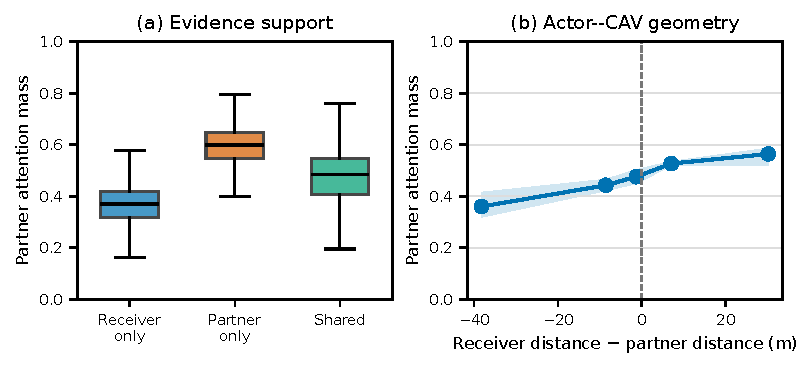
\includegraphics[width=0.78\textwidth]{dualcmp_attention_analysis}
\caption{Attention weights on the V2V4Real test set. (a) Partner attention mass for receiver-only, partner-only, and shared agents. The center line, box, and whiskers denote the median, interquartile range, and 1.5-IQR range, respectively. (b) Mean partner attention mass for five groups of relative agent--CAV distance. The shaded region denotes the 95\% confidence interval. A positive relative distance indicates that the agent is closer to the partner CAV.}
\label{fig:cooperative_analysis}
\end{figure*}

\subsection{Qualitative Results}

We provide qualitative results on the V2V4Real test set in Figure~\ref{fig:attention_examples}. We select one partner-only agent and one shared agent. Each selected agent has at least four observations, a complete 5-s future trajectory, and a future displacement of at least 5 m. In each group, we select the example whose 5-s minFDE$_6$ is closest to the group median. The fused-BEV panels show the objectness response and tracked state. The CAV panels show the agent-centered feature maps and the attention weights. The last panels show the observed trajectory, ground-truth trajectory, six predicted trajectories, and their probabilities.

\begin{figure*}[t]
\centering
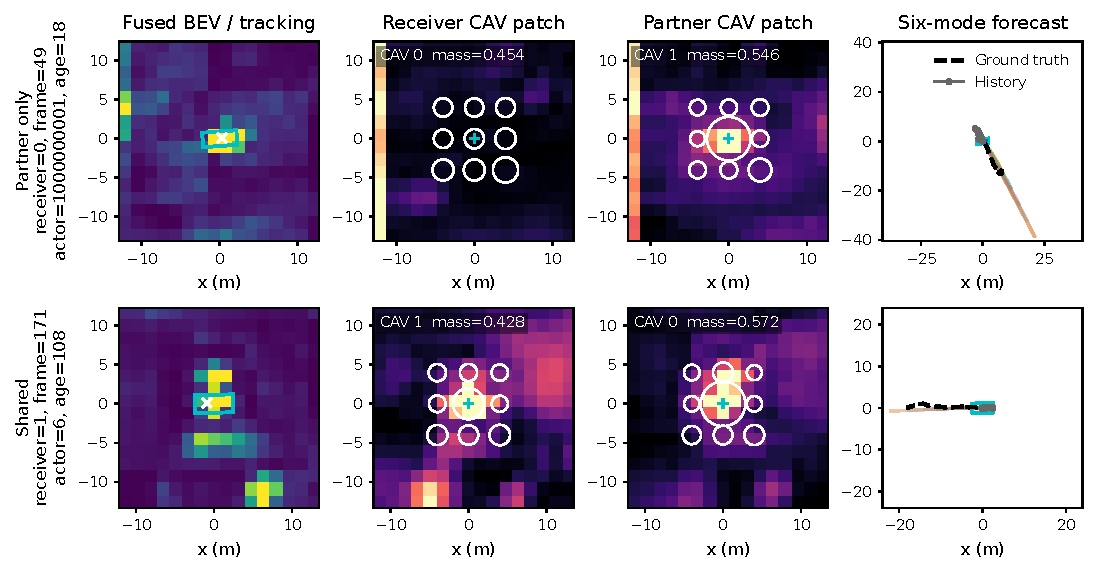
\includegraphics[width=\textwidth]{dualcmp_attention_examples}
\caption{Qualitative results of DualCMP on the V2V4Real test set. Each row shows one tracked agent. The first column shows the fused-BEV objectness response and tracked state. The second and third columns show the receiver-aligned CAV feature maps. Circle area represents the attention weight, and each panel reports the sum of the nine attention weights. The last column shows the observed trajectory in gray, the ground-truth trajectory as a black dashed line, and six predicted trajectories. The opacity of each predicted trajectory represents its probability.}
\label{fig:attention_examples}
\end{figure*}

\section{Conclusion}

This paper presented DualCMP, a LiDAR-based framework for cooperative tracking and motion prediction that assigns fused and source-specific BEV representations to different tasks. FuseBEVT supplies common current-state measurements to one persistent query bank, while receiver-aligned per-CAV features are sampled around each tracked agent and aggregated for forecasting. The resulting agent context is combined with ordered online histories, agent interactions, and motion anchors to produce six-mode 5-s trajectories without feeding predicted futures back into tracking. Under the strict-online V2V4Real protocol, the current seed-20 model obtains a 5-s minADE$_6$ of 1.9350 m and minFDE$_6$ of 3.2465 m while maintaining 65.04\% MOTA and 80.49\% forecast coverage. The learned source weights vary with observation support and relative CAV--agent distance, showing that source aggregation does not collapse to fixed averaging. A protocol-matched fused-BEV comparison and additional seeds are still required to determine whether the retained source representation provides a reproducible forecasting advantage. The current study is limited to two synchronous CAVs on one dataset; asynchronous communication and larger cooperative groups remain for future work.

\begin{thebibliography}{00}
\bibitem{xu2023v2v4real}
R.~Xu \emph{et al.}, ``V2V4Real: A Real-World Large-Scale Dataset for Vehicle-to-Vehicle Cooperative Perception,'' in \emph{Proc. IEEE/CVF Conf. Comput. Vis. Pattern Recognit.}, 2023.

\bibitem{wang2025cmp}
Z.~Wang \emph{et al.}, ``CMP: Cooperative Motion Prediction With Multi-Agent Communication,'' \emph{IEEE Robot. Autom. Lett.}, vol.~10, no.~4, pp.~3876--3883, 2025.

\bibitem{zhou2025v2xpnp}
Z.~Zhou \emph{et al.}, ``V2XPnP: Vehicle-to-Everything Spatio-Temporal Fusion for Multi-Agent Perception and Prediction,'' in \emph{Proc. IEEE/CVF Int. Conf. Comput. Vis.}, 2025.

\bibitem{souig2026unimm}
S.~Souig \emph{et al.}, ``UniMM-V2X: MoE-Enhanced Multi-Level Fusion for End-to-End Cooperative Autonomous Driving,'' in \emph{Proc. AAAI Conf. Artif. Intell.}, 2026.

\bibitem{zhou2023qcnet}
Z.~Zhou, J.~Wang, Y.-H.~Li, and Y.-K.~Huang, ``Query-Centric Trajectory Prediction,'' in \emph{Proc. IEEE/CVF Conf. Comput. Vis. Pattern Recognit.}, 2023.

\bibitem{zhou2022hivt}
Z.~Zhou \emph{et al.}, ``HiVT: Hierarchical Vector Transformer for Multi-Agent Motion Prediction,'' in \emph{Proc. IEEE/CVF Conf. Comput. Vis. Pattern Recognit.}, 2022.

\bibitem{pang2023pftrack}
Z.~Pang \emph{et al.}, ``Standing Between Past and Future: Spatio-Temporal Modeling for Multi-Camera 3D Multi-Object Tracking,'' in \emph{Proc. IEEE/CVF Conf. Comput. Vis. Pattern Recognit.}, 2023.

\bibitem{papais2025foresight}
S.~Papais \emph{et al.}, ``ForeSight: Multi-View Streaming Joint Object Detection and Trajectory Forecasting,'' in \emph{Proc. IEEE/CVF Int. Conf. Comput. Vis.}, 2025.

\bibitem{wang2020v2vnet}
T.-H.~Wang \emph{et al.}, ``V2VNet: Vehicle-to-Vehicle Communication for Joint Perception and Prediction,'' in \emph{Proc. Eur. Conf. Comput. Vis.}, 2020.

\bibitem{gu2023vip3d}
J.~Gu \emph{et al.}, ``ViP3D: End-to-End Visual Trajectory Prediction via 3D Agent Queries,'' in \emph{Proc. IEEE/CVF Conf. Comput. Vis. Pattern Recognit.}, 2023.

\bibitem{ruan2024v2xgraph}
H.~Ruan, H.~Yu, W.~Yang, S.~Fan, and Z.~Nie, ``Learning Cooperative Trajectory Representations for Motion Forecasting,'' in \emph{Adv. Neural Inf. Process. Syst.}, 2024.

\bibitem{you2025vitraj}
S.~You, L.~Weng, and F.~Gao, ``ViTraj: Learning Dual-Side Representations for Vehicle-Infrastructure Cooperative Trajectory Prediction,'' in \emph{Proc. ACM Multimedia}, 2025.

\bibitem{madjid2026latefusion}
N.~A.~Madjid \emph{et al.}, ``Collaborative Trajectory Prediction via Late Fusion,'' arXiv preprint arXiv:2604.22973, 2026.

\bibitem{yu2023v2xseq}
H.~Yu \emph{et al.}, ``V2X-Seq: A Large-Scale Sequential Dataset for Vehicle-Infrastructure Cooperative Perception and Forecasting,'' in \emph{Proc. IEEE/CVF Conf. Comput. Vis. Pattern Recognit.}, 2023.

\bibitem{wu2025copad}
K.~Wu, J.~Qiao, and Y.~Zhang, ``CoPAD: Multi-Source Trajectory Fusion and Cooperative Trajectory Prediction With Anchor-Oriented Decoder in V2X Scenarios,'' in \emph{Proc. IEEE/RSJ Int. Conf. Intell. Robots Syst.}, 2025.

\bibitem{zhang2025comtp}
X.~Zhang \emph{et al.}, ``Co-MTP: A Cooperative Trajectory Prediction Framework With Multi-Temporal Fusion for Autonomous Driving,'' in \emph{Proc. IEEE Int. Conf. Robot. Autom.}, 2025.

\bibitem{shi2022mtr}
S.~Shi \emph{et al.}, ``Motion Transformer With Global Intention Localization and Local Movement Refinement,'' in \emph{Adv. Neural Inf. Process. Syst.}, 2022.
\end{thebibliography}

\end{document}
